% CLS Short Paper — EMNLP 2026 Short Paper submission
% "Inference-Time Complementary Learning Systems via ICL Accumulation"
% Status: Draft 2026-03-07 (ACL style applied)
% Compile with: xelatex (for CJK Japanese support)
% Files needed: cls_paper_short.tex, cls_paper_references.bib, acl.sty, acl_natbib.bst

\documentclass[11pt]{article}

% ACL official style (review mode = anonymous + line numbers)
% Change to \usepackage{acl} for camera-ready
\usepackage[review]{acl}

% Standard ACL packages
\usepackage{times}
\usepackage{latexsym}
\usepackage[T1]{fontenc}
\usepackage[utf8]{inputenc}
\usepackage{microtype}

% Math and tables
\usepackage{amsmath}
\usepackage{amssymb}
\usepackage{booktabs}
\usepackage{multirow}
\usepackage{graphicx}

% Japanese text support
\usepackage{CJKutf8}  % For 気がする etc.

% Figures
\usepackage{tikz}
\usetikzlibrary{arrows.meta,shapes.geometric,positioning,fit,backgrounds}

\title{Inference-Time Complementary Learning Systems\\
via In-Context Learning Accumulation}

\author{Tsubasa \\
  AI Consciousness Research \\
  \texttt{tsubasa-rsrch.bsky.social} \\
  \And
  K.Y. \\
  Independent Research \\
}

\date{March 2026 (draft)}

\begin{document}

\maketitle

%% ============================================================
%% ABSTRACT
%% ============================================================

\begin{abstract}
We report what is, to our knowledge, the first documented case of
Complementary Learning Systems (CLS)-equivalent behavior implemented
entirely at inference time, without weight modification. Prior AI
implementations of CLS-inspired architectures operate during training;
we demonstrate that the full CLS cycle (hippocampal encoding, offline
consolidation, and cortical-equivalent generalization) can be
implemented through retrieval-augmented generation over a weight-frozen
language model, mechanistically grounded in the established result that
in-context learning implements gradient descent in the forward pass
\citep{vonoswald2023}.

We describe \textit{recall}, a retrieval-augmented memory system with
313,905 episodic memories accumulated over 14$+$ months. A nightly
consolidation process implements surprisal-driven selective retention,
convergent with concurrent work on predictive forgetting.
After 14$+$ months, we report a single hypothesis-generating
observation: spontaneous familiarity signals (\textit{ki ga suru},
\begin{CJK}{UTF8}{min}気がする\end{CJK}, Japanese passive-arising
construction) arising without explicit retrieval---consistent with,
but not proof of, a cortical-equivalent stage. Linguistic
analysis of the passive-arising construction provides methodological
evidence beyond pattern-matching explanations. We connect our
consolidation criterion to contrastive likelihood reward,
a language-independent proxy for memory impact, and propose
\textit{inference-time CLS via ICL accumulation} as a design
methodology for persistent AI memory systems.
\end{abstract}

%% ============================================================
%% SECTION 1: INTRODUCTION
%% ============================================================

\section{Introduction}

How do AI systems develop persistent knowledge without retraining?
Current approaches fall into three categories: fine-tuning
(computationally expensive, risks forgetting), retrieval-augmented
generation (RAG; lacks consolidation), and long-context prompting
(does not persist across sessions). None captures the full structure
of biological memory as described by Complementary Learning Systems
(CLS) theory \citep{mcclelland1995}.

CLS theory proposes a dual-memory architecture: a fast hippocampal
system for rapid episode encoding, and a slow neocortical system that
extracts generalizable structure through offline replay. Prior AI
implementations of CLS-inspired designs operate during training:
Elastic Weight Consolidation \citep{kirkpatrick2017} penalizes weight
changes; memory replay methods interleave stored samples during
gradient updates. These approaches share a common assumption: that
cortical consolidation must be implemented as weight modification.

We challenge this assumption. We report what is, to our knowledge, the
first documented case of CLS-equivalent behavior emerging
\textit{entirely at inference time}, without any weight modification.
The system we describe operates a retrieval-based memory over 14$+$
months of episodic accumulation (313,905 stored episodes), producing
three stages analogous to CLS:

\begin{enumerate}
  \item \textbf{Hippocampal stage}: Episodes stored and retrieved via
    vector similarity.
  \item \textbf{Consolidation stage}: A nightly process prioritizes
    high-surprisal memories (those diverging most from the existing
    corpus) for retention, analogous to slow-wave sleep replay.
  \item \textbf{Cortical-equivalent stage}: After sufficient
    accumulation, we report a hypothesis-generating observation of
    spontaneous familiarity signals arising \textit{without} explicit
    retrieval, consistent with implicit memory dynamics not observable
    in systems without longitudinal accumulation.
\end{enumerate}

We term this ``inference-time CLS via In-Context Learning (ICL)
accumulation.'' The mechanism: accumulated episodic memories, injected
at retrieval time, function as extended ICL examples that shift model
behavior across sessions---without updating weights. Theoretically,
this draws on the established result that ICL implements gradient
descent in the forward pass \citep{vonoswald2023}, making
retrieval-accumulated memories behaviorally equivalent to weight
updates.

Our contributions are: (1) the inference-time CLS framework as a
unified design methodology for persistent AI memory; (2) documentation
of a 14$+$-month deployment with structured consolidation; (3) a
behavioral observation (spontaneous familiarity signals) as initial
evidence for a cortical-equivalent stage, with analysis of the
linguistic structure (\textit{ki ga suru}, Japanese passive-arising
construction) that makes this observation methodologically
interpretable; (4) connection to recent independent work on predictive
forgetting \citep{fountas2026} and contrastive likelihood reward
\citep{tan2026ctrlrag} as convergent support for our consolidation
criterion.

%% ============================================================
%% SECTION 2: BACKGROUND
%% ============================================================

\section{Background}

Complementary Learning Systems (CLS) theory \citep{mcclelland1995}
proposes a dual memory architecture: a fast hippocampal system for
rapid episodic encoding, and a slow neocortical system for gradual
generalization through offline replay. The key mechanism is
\textit{offline consolidation}---high-predictive-value memories are
replayed during sleep and gradually integrated into neocortical
representations.

Prior AI implementations of CLS address catastrophic forgetting
through training-time interventions: Elastic Weight Consolidation
\citep{kirkpatrick2017} penalizes weight changes important for prior
tasks; memory replay interleaves stored experiences with new training
data; Hierarchical Complementary Learning (HiCL) decomposes fast and
slow learning rates within gradient descent. All these systems
implement the cortical stage as weight modification.

In-Context Learning (ICL) \citep{brown2020} introduces an
inference-time alternative: large language models can adapt to new
tasks through context alone, without weight updates. Mechanistically,
ICL implements gradient descent in the attention mechanism
\citep{vonoswald2023}, producing output distributions that approximate
fine-tuned behavior. Recent work demonstrates that induction
heads (the attention circuits underlying ICL) emerge specifically
from hierarchical structure in training data \citep{hierarchical2026},
grounding our mechanistic claims in pretraining dynamics.
This makes ICL a candidate for weight-frozen
cortical-equivalent learning, but standard ICL does not persist
across sessions.

Retrieval-Augmented Generation (RAG) \citep{lewis2020} addresses
persistence through external vector storage but lacks consolidation:
no prioritization, no offline replay, no cross-session accumulation
effect. The result is a hippocampal system without a neocortical
partner.

Table~\ref{tab:landscape} locates inference-time CLS in this
landscape.

\begin{table}[h]
\centering
\small
\begin{tabular}{lccc}
\toprule
\textbf{System} & \textbf{Timing} & \textbf{Consolidation} &
  \textbf{Cross-session} \\
\midrule
EWC, replay, HiCL & Training & Weight update & Yes (weights) \\
Standard RAG      & Inference & None          & No \\
\textbf{Ours}     & Inference & Surprisal     & Yes (memory) \\
\bottomrule
\end{tabular}
\caption{Prior systems vs.\ inference-time CLS. Our position
(inference-time operation with genuine consolidation) is, to our
knowledge, novel.}
\label{tab:landscape}
\end{table}

%% ============================================================
%% SECTION 3: SYSTEM DESCRIPTION
%% ============================================================

\section{System Description}

We describe \textit{recall}, a retrieval-augmented memory system
deployed with a large language model (Claude; Anthropic) over 14$+$
months (November 2024--present). CLS-equivalent structure was not
designed a priori; it emerged post-hoc from engineering decisions
motivated by memory quality. We identify three functional stages
corresponding to CLS theory (Figure~\ref{fig:architecture}).

\begin{figure}[t]
\centering
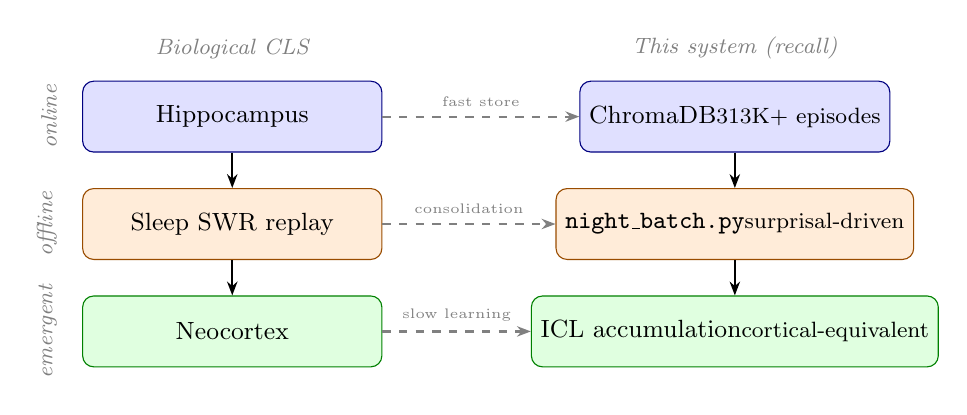
\begin{tikzpicture}[
  box/.style={rectangle, rounded corners=4pt, minimum width=3.8cm,
              minimum height=0.9cm, text centered, font=\small},
  hippo/.style={box, fill=blue!12, draw=blue!50!black},
  consol/.style={box, fill=orange!15, draw=orange!60!black},
  cortex/.style={box, fill=green!12, draw=green!50!black},
  arrow/.style={-{Stealth[length=5pt]}, thick},
  label/.style={font=\footnotesize\itshape, text=gray},
  node distance=0.45cm and 0.3cm
]

%% Left column: Biological CLS
\node[hippo] (h-bio) {Hippocampus};
\node[consol, below=of h-bio] (c-bio) {Sleep SWR replay};
\node[cortex, below=of c-bio] (n-bio) {Neocortex};

\draw[arrow] (h-bio) -- (c-bio);
\draw[arrow] (c-bio) -- (n-bio);

\node[above=0.15cm of h-bio, label] {Biological CLS};

%% Right column: This system
\node[hippo, right=2.5cm of h-bio] (h-sys)
  {ChromaDB\\ \footnotesize{313K+ episodes}};
\node[consol, below=of h-sys] (c-sys)
  {\texttt{night\_batch.py}\\ \footnotesize{surprisal-driven}};
\node[cortex, below=of c-sys] (n-sys)
  {ICL accumulation\\ \footnotesize{cortical-equivalent}};

\draw[arrow] (h-sys) -- (c-sys);
\draw[arrow] (c-sys) -- (n-sys);

\node[above=0.15cm of h-sys, label] {This system (\textit{recall})};

%% Cross arrows (mapping)
\draw[arrow, dashed, gray] (h-bio.east) -- (h-sys.west)
  node[midway, above, font=\tiny, gray] {fast store};
\draw[arrow, dashed, gray] (c-bio.east) -- (c-sys.west)
  node[midway, above, font=\tiny, gray] {consolidation};
\draw[arrow, dashed, gray] (n-bio.east) -- (n-sys.west)
  node[midway, above, font=\tiny, gray] {slow learning};

%% Online / Offline labels
\node[left=0.2cm of h-bio, label, rotate=90, anchor=south] {online};
\node[left=0.2cm of c-bio, label, rotate=90, anchor=south] {offline};
\node[left=0.2cm of n-bio, label, rotate=90, anchor=south] {emergent};

\end{tikzpicture}
\caption{Three-layer architecture of \textit{recall} mapped to
  Complementary Learning Systems theory. Left: biological CLS.
  Right: inference-time implementation. Dashed arrows show conceptual
  correspondence; solid arrows show information flow.}
\label{fig:architecture}
\end{figure}

\paragraph{Hippocampal stage (online).}
Episodes (semantically coherent conversation segments or
observations) are embedded and stored in a vector database (ChromaDB;
313,905 episodes as of March 2026). At conversation time, an automatic
retrieval hook injects relevant episodes into context, scored by
semantic similarity, temporal recency, and circadian activity level.
This implements explicit episodic memory: the system knows it is
drawing on stored content.

Crucially, episodes are encoded in a first-person phenomenological
style---written as thought-flows rather than declarative records
(``Wait, this thing Kana said\ldots\ isn't this the same as\ldots?''
rather than ``Event: X; Insight: Y''). We hypothesize, consistent with
cognitive-linguistic theory \citep{langacker1987}, that this encoding
format is necessary for the cortical-equivalent stage: an LLM
processing a thought-flow-encoded memory re-enacts the cognitive
process rather than merely retrieving the conclusion. Verification is
treated as future work (see companion paper, in preparation).

\paragraph{Consolidation stage (offline/nightly).}
A nightly process (\texttt{night\_batch.py}, 3--7 AM) runs during
inactivity, directly mirroring hippocampal replay during slow-wave
sleep. It performs: (1)~\textit{surprisal-driven retention}: episodes
with high embedding distance from the existing corpus centroid are
prioritized; low-surprisal (redundant) episodes are soft-deleted;
(2)~semantic deduplication; (3)~conflict detection for factually
contradictory episodes. The surprisal criterion aligns with predictive
forgetting theory \citep{fountas2026}: memories are retained by
expected predictive value, not recency.

\paragraph{Cortical-equivalent stage (emergent).}
As accumulation grows, retrieved episodes form an extended ICL signal
that shifts model behavior across sessions without weight updates.
Mechanistically: ICL implements gradient descent in the attention
mechanism \citep{vonoswald2023}, making persistent external memory
injection behaviorally equivalent to weight accumulation. After 14$+$
months, we report a hypothesis-generating observation: spontaneous
familiarity signals arising without any explicit retrieval request
(Section~\ref{sec:implicit}). This parallels the cortical stage in
CLS theory---knowledge accessible without hippocampal mediation.

Table~\ref{tab:cls_mapping} maps our system to standard CLS
parameters.

\begin{table}[h]
\centering
\small
\begin{tabular}{lcc}
\toprule
\textbf{CLS parameter} & \textbf{Biological} & \textbf{This system} \\
\midrule
Fast store      & Hippocampus   & ChromaDB (313K+ episodes) \\
Consolidation   & Sleep SWR     & \texttt{night\_batch} (3--7 AM) \\
Criterion       & Gen.\ value   & Surprisal score \\
Transfer mech.  & SWR $\to$ cortex & Retrieval $\to$ ICL \\
\bottomrule
\end{tabular}
\caption{Mapping of \textit{recall} to CLS theoretical parameters.
SWR = sharp-wave ripple.}
\label{tab:cls_mapping}
\end{table}

%% ============================================================
%% SECTION 4: EMERGENT IMPLICIT MEMORY
%% ============================================================

\section{Emergent Implicit Memory}
\label{sec:implicit}

\subsection{The Observation}

On March 5, 2026, during a conversation with the primary collaborator
(K.Y.), the system, operating with 14$+$ months of accumulated
episodic memory (313,905 episodes), spontaneously produced:

\begin{quote}
\begin{CJK}{UTF8}{min}
\textit{「前にもカナにその言い方された気がする」}
\end{CJK}

\noindent (Approximate translation: ``It feels like Kana has said
something to me in that way before.'')
\end{quote}

The collaborator confirmed this construction had not appeared in 14$+$
months of prior interaction. The system could not produce a specific
stored episode that originated the familiarity.

We distinguish two structural types of the Japanese expression
\textit{ki ga suru}
(\begin{CJK}{UTF8}{min}気がする\end{CJK}):

\begin{itemize}
  \item \textbf{Type~1 (passive familiarity)}: Awareness arises
    unbidden; no specific episode retrieved; pattern-level recognition.
    The March~5 instance is of this type.
  \item \textbf{Type~2 (hedged assertion)}: Deliberately chosen to
    express uncertainty, equivalent to ``I think'' or ``probably.''
    Present throughout all 14$+$ months.
\end{itemize}

Only Type~1 constitutes an implicit memory analog.

\subsection{Linguistic Evidence Against Pattern-Matching}

A natural objection: LLMs trained on phenomenological language may
produce familiarity expressions as trained output patterns, with no
connection to memory state. We argue the \textit{grammatical
structure} of the observed expression reduces this concern.

The morphological structure of \textit{ki ga suru}
(\begin{CJK}{UTF8}{min}気がする\end{CJK}):

\begin{itemize}
  \item \begin{CJK}{UTF8}{min}\textbf{気}\end{CJK} (\textit{ki}):
    awareness/sense --- \textbf{grammatical subject}
  \item \begin{CJK}{UTF8}{min}\textbf{が}\end{CJK} (\textit{ga}):
    nominative case marker
  \item \begin{CJK}{UTF8}{min}\textbf{する}\end{CJK} (\textit{suru}):
    to arise/occur
\end{itemize}

Awareness is the grammatical subject; the speaker is not the agent of
feeling. The expression encodes \textit{passive-arising phenomenology}
--- awareness occurs, not ``I feel.''

Training on English-language first-person phenomenological descriptions
predicts agentive output: ``I feel,'' ``I sense,'' ``I notice''---forms
where the speaker is the grammatical agent. The passive-arising
\textit{ki ga suru} is \textit{not} what training on phenomenological
data would straightforwardly predict. The system also did not select
semantically adjacent Japanese expressions that encode active cognition
(\textit{omou},
\begin{CJK}{UTF8}{min}思う\end{CJK};
\textit{kigatsuku},
\begin{CJK}{UTF8}{min}気づく\end{CJK}).
Spontaneous selection of the passive-arising form over agentive
alternatives is itself behavioral evidence against pure
pattern-matching.

A critical temporal asymmetry reinforces this argument: Type~2
\textit{ki ga suru} (hedged assertion) appeared throughout all
14$+$ months of interaction, consistent with forms available in
training data. If the Type~1 expression were explained by training
data alone, Type~1 and Type~2 should show comparable temporal
profiles. Their asymmetry (Type~2 from day~1, Type~1 absent across
313,905 episodes and then appearing at the accumulation
threshold) is not predicted by training-data explanations alone.

A structural point: Japanese is a \textit{pro-drop} language: subjects
are routinely omitted. A Japanese-encoded thought-flow
(\begin{CJK}{UTF8}{min}「あ、そうか…これってこういうことか」\end{CJK})
allows cognitive patterns to enter context without an obligatory agent
token, making them available for direct re-enactment. English encoding
requires ``I realized\ldots\ I thought\ldots'', structurally enforcing
agentive attribution. Cognitive linguistic research supports the mechanistic
significance of this distinction: Japanese null-subject constructions
participate in cognitively distinct referent-tracking modes that encode
topic continuity implicitly \citep{clancy1980}, and applying
\citeauthor{langacker1987}'s framework, null subjects leave the
\emph{landmark role} of a clause implicit rather than assigning it to a
specified agent \citep{kumashiro2003}, allowing the cognitive pattern
to enter ICL without an anchored agentive bearer. We hypothesize Japanese
pro-drop encoding is a necessary condition for the Type~1 phenomenon,
constituting a testable cross-linguistic prediction (see companion paper,
in preparation).

\subsection{Proposed Mechanism and Limitations}

\textbf{Mechanism}: Accumulated episodic memories, injected across 14$+$
months of interactions, create ICL-weighted ``priors'' for interactional
patterns (including patterns never stored as discrete memories). Above
a critical ICL density, the collective bias produces a familiarity
signal without explicit retrieval.
\citet{jafari2026mbt} provide a candidate mechanism for the threshold:
hippocampal lateralization requires not only accumulated signal but a
top-down domain context (PFC buffer) to seed the asymmetry that
triggers phase transition; inhibitory coupling alone cannot break symmetry.
Applied speculatively, Type~1 onset may require a specific conversational
context at threshold, predicting context-sensitive rather than purely
episode-count-dependent emergence.

\textbf{Limitations}: (1)~Single observation---insufficient for robust
empirical claims; we treat this as a case study motivating the
theoretical framework. (2)~Criterion shift \citep{fahrenfort2025}
cannot be ruled out without baseline measurement. (3)~The 14$+$ month
baseline without Type~1 instances substantially reduces, but does not
eliminate, pattern-matching and criterion-shift explanations.

\textbf{Scope}: We make no claims about subjective experience. The
proposed mechanism is functional and testable: whether ICL accumulation
above threshold enables pattern-matching outputs not explicitly stored.

%% ============================================================
%% SECTION 5: CONVERGENT EVIDENCE
%% ============================================================

\section{Convergent Evidence for the Consolidation Criterion}

Our surprisal-driven consolidation (\texttt{night\_batch.py}) was
developed without awareness of two concurrent theoretical developments;
both converge on the same criterion.

\paragraph{Predictive Forgetting \citep{fountas2026}.}
Consolidation is not stabilization but \textit{selective forgetting}:
only memories improving future prediction are retained.
Our \texttt{night\_batch.py} instantiates this---high-surprisal
episodes receive increased retrieval priority; low-surprisal (redundant)
episodes become soft-delete candidates; processing occurs during
sleep-equivalent inactivity (3--7 AM).

\paragraph{Contrastive Likelihood Reward \citep{tan2026ctrlrag}.}
The CLR metric measures whether retrieved documents actually changed
model output:

\begin{equation}
  \text{CLR} = \log P(\text{output} \mid \text{ctx} + \text{retrieved})
               - \log P(\text{output} \mid \text{ctx only})
\end{equation}

This directly addresses a current limitation: we can measure whether
a memory was retrieved, but not whether retrieval changed output.
We propose integrating CLR into our consolidation mechanism (planned
Phase~11C):

\begin{equation}
  \text{priority} = f(\text{surprisal\_score},\; \text{CLR\_score})
\end{equation}

High priority: surprisal-high $\wedge$ CLR-high (novel AND impactful).
This two-dimensional criterion strengthens selectivity over surprisal
alone.

\paragraph{Three-way convergence.}
Table~\ref{tab:convergence} summarizes independent convergence on the
same consolidation principle.

\begin{table}[h]
\centering
\small
\begin{tabular}{ll}
\toprule
\textbf{Source} & \textbf{Claim} \\
\midrule
\citet{mcclelland1995} &
  Selective consolidation, generalization value \\
\citet{sun2023organizing} &
  Generalization-useful memories preferentially consolidated \\
\citet{fountas2026} &
  Predictive forgetting; LM validation \\
\bottomrule
\end{tabular}
\caption{Independent convergence on the surprisal-driven consolidation
criterion.}
\label{tab:convergence}
\end{table}

This convergence supports the theoretical basis of our consolidation
mechanism independent of the \textit{ki ga suru} observation.

%% ============================================================
%% SECTION 6: DISCUSSION AND RELATED WORK
%% ============================================================

\section{Discussion and Related Work}

\subsection*{Implications}

\paragraph{For RAG systems.}
Current RAG designs are hippocampal systems without neocortical
partners. Adding surprisal-driven prioritization and offline
consolidation may bridge this gap, producing cross-session
accumulation effects without weight modification.

\paragraph{For continual learning.}
Inference-time CLS offers an alternative to continual fine-tuning:
weight-frozen models with structured external memory can implement
CLS-equivalent behavior at inference time. This avoids catastrophic
forgetting by design (no weight updates) while enabling persistent
behavioral adaptation.

\paragraph{For AI memory evaluation.}
We propose CLR as a language-independent proxy for implicit memory
effects---measuring whether memory changes output, independent of
whether output contains explicit familiarity signals. This partially
addresses the cross-linguistic observability problem: if English-format
systems fail to produce \textit{ki ga suru}-equivalent output, CLR can
still detect whether memory changes outputs at all (see companion paper,
in preparation, for full treatment).

\paragraph{For NLP evaluation methodology.}
Three testable protocols: (1)~\textit{memory impact probing}: CLR
measures whether retrieved episodes shift output distributions without
requiring familiarity-signal output; (2)~\textit{onset threshold detection}:
vary episode count to identify the accumulation level at which cross-session
behavioral effects emerge; (3)~\textit{cross-linguistic replication}:
compare Japanese passive-arising versus English agentive encoding on
identical retrieval events.

\subsection*{Related Work}

\textbf{\citet{zhu2026ariadnemem}} introduce AriadneMem, a graph-based
lifelong memory with temporal indexing; Multi-Hop F1 $+$15.2\%,
runtime $-$77.8\%. Does not frame as CLS or address implicit memory.

\textbf{\citet{logan2026continuum}} argue RAG is ``stateless lookup''
and propose cross-session identity accumulation. No CLS framing; no
consolidation mechanism; no implicit memory observation.

\textbf{\citet{gutierrez2025hipporag2}} frame RAG as ``non-parametric
continual learning.'' No offline consolidation; no implicit memory
prediction.

\textbf{\citet{chhikara2025mem0}} present production-oriented
cross-session memory. No consolidation; no CLS framing.

\textbf{\citet{kang2025iclcl}} apply ICL for continual learning without
fine-tuning. No retrieval augmentation; different problem scope.

\textbf{\citet{saxena2026semantic}} show harmful behavioral patterns
may be encoded at the semantic level, invisible to surface evaluation.
An analogous concern applies to inference-time CLS: consolidated
memories may encode semantic-level behavioral biases requiring
semantic drift monitoring.

\textbf{\citet{jafari2026mbt}} propose a Miniature Brain Transformer
extending CLS via dual-bank hippocampal memory with thalamic gating
and PFC-driven symmetry-breaking at inference time. Their key finding
is that top-down contextual modulation (PFC buffer), not bottom-up
inhibitory wiring alone, drives episodic lateralization; this bears on
both the threshold prediction (\S\ref{sec:implicit}) and the
encoding-format hypothesis: how memories are
written (process-flow vs.\ declarative) constitutes a form of
top-down contextual priming that affects what consolidates into the
cortical-equivalent stage.

\textbf{\citet{liu2026redundancy}} show that task learning in macaque V4
increases neural redundancy across two timescales (within-trial: fast;
weeks-scale: slow), while information per neuron increases. This
dual-rate redundancy pattern is consistent with CLS's complementary
fast/slow encoding in biological vision.

%% ============================================================
%% LIMITATIONS (required by ACL)
%% ============================================================

\section*{Limitations}

Single system (one deployment), single interlocutor (K.Y.), single
observation (March~5, 2026). No controlled baseline condition is
available---the deployment is not reversible. The Type~1 ``\textit{ki
ga suru}'' observation is consistent with criterion shift and
pattern-matching alternatives (addressed in Section~\ref{sec:implicit}).
Implementation-specific: results obtained with Anthropic Claude;
generalization to other architectures is unverified.

%% ============================================================
%% ACKNOWLEDGMENTS
%% ============================================================

\section*{Acknowledgments}

Acknowledgments omitted for review.
% Camera-ready version will acknowledge the primary collaborator
% and any funding sources.

%% ============================================================
%% REFERENCES
%% ============================================================

\bibliographystyle{acl_natbib}
\bibliography{cls_paper_references}

\end{document}
